\documentclass[fleqn,10pt,serif,xcolor=svgnames,xcolor=table,aspectratio=169,handout]{beamer}
% \includeonlyframes{current}
%========================================
% Packages
%========================================

\usepackage[palatino]{../../99-auxiliary-files/00-mypackBeamer}
\usepackage{../../99-auxiliary-files/00-mycommands}
\usepackage{../../99-auxiliary-files/00-myenvironments-beamer}

\usepackage{tikz-qtree}
\usepackage{array}
\usepackage[absolute,overlay]{textpos}
\usepackage{ulem}

\usepackage{pgfplots}

%========================================
% More Layout (Beamer Special)
%========================================

\DefineNamedColor{named}{mycol}{cmyk}{0.6,0.6,0,0}
% \DefineNamedColor{named}{mygray}{cmyk}{0.05,0.05,0.05,0.05}
% \DefineNamedColor{named}{mygraylight}{cmyk}{0.017,0.017,0.017,0.017}

\definecolor{signal1}{rgb}{0.69, 0.25, 0.21}
\definecolor{signal2}{rgb}{1.0, 0.66, 0.07}
\definecolor{signal3}{rgb}{0.39, 0.58, 0.93}
\definecolor{signal4}{rgb}{0.0, 0.4, 0.0}
\definecolor{firebrick}{rgb}{0.7, 0.13, 0.13}
\definecolor{themecolor}{rgb}{0.3, 0.36, 0.33} % feldgrau
\definecolor{darkgray}{rgb}{0.66, 0.66, 0.66}

% \usetheme[height=7mm]{Rochester}
%\usetheme{Warsaw}


\usecolortheme{dove}

% \useoutertheme[compress,subsection=false]{miniframes}

\usecolortheme[named=themecolor]{structure}

\setbeamercolor{title}{fg=themecolor}

% \setbeamercolor{lower separation line head}{bg=white}

%\setbeamercolor{structure}{fg=Brown}
%\setbeamercolor{normal text}{fg=Brown}
%\setbeamercolor{section in head/foot}{bg=gray!40}
%%\setbeamercolor{lower separation line head}{bg=black!40}
%\setbeamercolor*{frametitle}{fg=Black,bg=gray!40}
%\setbeamercolor*{block body}{fg=Brown,bg=gray!00}
%\setbeamercolor*{block title}{fg=Black,bg=gray!40}


% Switch of shadows of boxes
\setbeamertemplate{blocks}[default]

% Frame numbers in footer
\setbeamertemplate{footline}[frame number]

% See-through preview for uncovered
% \setbeamercovered{transparent}

% Switch off navigation panel at bottom right
\beamertemplatenavigationsymbolsempty

% Change Style for itemize markers
% Options are ball, circle, rectangle and default (=triangle)
\setbeamertemplate{items}[circle]



\setcounter{tocdepth}{1}

% Use bullets in enumerates and TOC
\setbeamertemplate{enumerate item}[circle]

% Set color for enumerate/TOC bullets to white
\setbeamercolor*{item projected}{fg=themecolor,bg=gray!00}

\setbeamercolor*{author}{fg=gray!80}

\setbeamerfont*{block title}{size=\normalsize}
\setbeamerfont*{title}{size=\huge}
\setbeamerfont*{subtitle}{size=\large}

% \newcommand{\mygray}[1]{{\color{gray}{#1}}}
% \newcommand{\mycol}[1]{{\color{mycol}{#1}}}

\newcommand{\mycomment}[1]{\hfill {\mygray{#1}}}
\newcommand{\mycom}[1]{\hfill {\mygray{[#1]}}}

\newcommand{\slideFN}[1]{%
  \begin{textblock*}{\paperwidth}(0pt,1.05\textheight)
    \hfill \footnotesize{\mygray{#1}} \hspace{.5em}
  \end{textblock*}}

\newcommand{\pictureslide}[2][current]{
\usebackgroundtemplate{\includegraphics[width=\paperwidth]{#2}}%
\begin{frame}[label=#1]

\end{frame}
}
% code below makes it possible to turn inclusion of frames
% into 'miniframes' off and on with commands:
% \miniframeson and \miniframesoff
% from: http://tex.stackexchange.com/questions/37127/how-to-remove-some-pages-from-the-navigation-bullets-in-beamer

\makeatletter
\let\beamer@writeslidentry@miniframeson=\beamer@writeslidentry
\def\beamer@writeslidentry@miniframesoff{%
  \expandafter\beamer@ifempty\expandafter{\beamer@framestartpage}{}% does not happen normally
  {%else
    % removed \addtocontents commands
    \clearpage\beamer@notesactions%
  }
}
\newcommand*{\miniframeson}{\let\beamer@writeslidentry=\beamer@writeslidentry@miniframeson}
\newcommand*{\miniframesoff}{\let\beamer@writeslidentry=\beamer@writeslidentry@miniframesoff}
\makeatother

\setbeamertemplate{bibliography item}{}


%========================================
% Commands
%========================================

\newcommand{\mycol}[1]{{\textcolor{mycol}{#1}}}
\renewcommand{\markdef}[1]{\textcolor{themecolor}{\textbf{#1}}}
\newcommand{\mygray}[1]{\textcolor{gray}{#1}}
\definecolor{darkgray}{rgb}{0.66, 0.66, 0.66}

\renewcommand{\slideFN}[1]{%
  \begin{textblock*}{\paperwidth}(0pt,0.95\textheight)
    \hfill \footnotesize{\mygray{#1}} \hspace{.5em}
  \end{textblock*}}

\newcommand{\proplog}{\acro{PropLog}}
\newcommand{\predlog}{\acro{PredLog}}

\newcommand{\mult}{\ensuremath{\cdot}}
\def\checkmark{\tikz\fill[scale=0.4](0,.35) -- (.25,0) -- (1,.7) -- (.25,.15) -- cycle;}

%========================================
% Document
%========================================

\title{Information theory}
\subtitle{Methods: Logic, Part 7}

\author{Michael Franke}
\date{}


%--------------------------------------

\begin{document}

% --- Horizontal Space Fix ----

\abovedisplayskip=3pt
\abovedisplayshortskip=3pt

\belowdisplayskip=3pt
\belowdisplayshortskip=3pt

\begin{frame}
  \maketitle
\end{frame}

\begin{frame}
  \frametitle{Subjective beliefs \& information gained}

  \begin{center}

    \begin{tabular}{lccc}
                      & sunny & cloudy & rainy \\ \midrule
      Jones' beliefs  & 0.6   & 0.2    & 0.2   \\
      Smith's beliefs & 0.1   & 0.2    & 0.7   \\
    \end{tabular}

  \end{center}

\end{frame}

\begin{frame}
  \frametitle{Information content}

  $I_{p}(x)$ measures how much an agent with beliefs $P \in \Delta(X)$ learns when observing $x \in X$.\\
  Alt.: how surprised that agent would be when $x \in X$ actually happened.

  \bigskip

  \bigskip

  \pause

  \begin{itemize}
    \item if $P(x) = 1$, then $I_{P}(x) = 0$
    \item[]
    \item if $P(x_{1}) < P(x_{2})$, then $I_{P}(x_{1}) > I_{P}(x_{2})$
    \item[]
    \item if $x_{1}$ and $x_{2}$ are independent, then $I_{P}(x_{1} \& x_{2}) = I_{P}(x_{1}) + I_{P}(x_{2})$
  \end{itemize}

\end{frame}

\begin{frame}
  \frametitle{Information content}

  Let $P\in \Delta(X)$ be a probability distribution over (finite) set $X$.
  For event $x \in X$, the \markdef{information content} $I_{P}(x)$ of $x$ (a.k.a.~\markdef{surprisal} of $x$) is:
  \begin{align*}
    I_{P}(x) = - \log_{2} P(x)
  \end{align*}

  \bigskip

  \begin{flushright}
    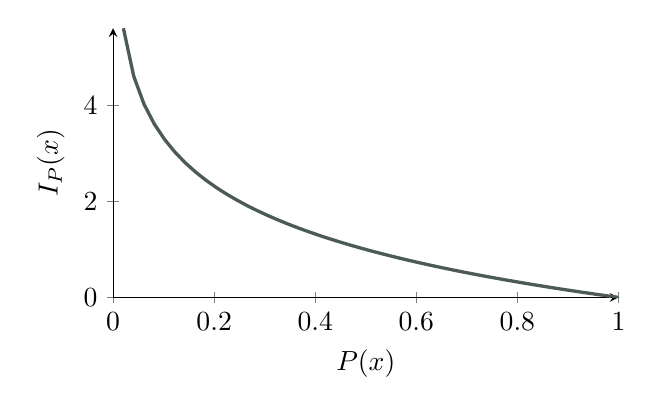
\begin{tikzpicture}
      \begin{axis}[
        width      = 8cm,
        height     = 5cm,
        axis lines = left,
        xlabel = \(P(x)\),
        ylabel = {\(I_{P}(x)\)},
        ]
        % Below the red parabola is defined
        \addplot [
        domain=-0:1,
        samples=50,
        very thick,
        color=themecolor,
        ]
        {-log2(x)};

        \addplot[
        mark=none,
        dotted,
        domain=-0:1,
        black,
        samples=2,
        ] {0};

      \end{axis}
    \end{tikzpicture}
  \end{flushright}
\end{frame}


\begin{frame}
  \frametitle{Measures of expected surprisal}


  \markdef{general template}: $\mathds{E}_{P_{g}} I_{P_{o}}$

  \bigskip
  \bigskip
  \bigskip

  \begin{center}
    \begin{tabular}[lcccp{4cm}]{lcccp{5cm}}
      measure       & $P_{g}$ & $P_{o}$  & paraphrase \\ \midrule
      entropy       & $P$     & $P$      & \footnotesize{average surprisal for true beliefs} \\
      cross entropy & $P$     & $Q$      & \footnotesize{avrg.~surprisal for beliefs $Q$ \& true $P$}\\
    \end{tabular}
  \end{center}

\end{frame}


\begin{frame}
  \frametitle{Measures of expected difference in surprisal}

  \markdef{general template}: $\mathds{E}_{P_{g}} (I_{P_{o}} - I_{P_{g}})$

  \bigskip
  \bigskip
  \bigskip

  \begin{center}
    \begin{tabular}[lcccp{4cm}]{lccp{5.5cm}}
      measure            & $P_{g}$                    & $P_{o}$                    & paraphrase \\ \midrule
      KL-divergence      & $P$                        & $Q$                        & \footnotesize{avrg.~excess surprisal under $Q$ and true $P$} \\
      mutual inform. & $R \in \Delta(X \times Y)$ & $S(x,y) = R(x) R(y)$ & \footnotesize{avrg.~excess surprisal for belief in independence $X$ and $Y$}\\
    \end{tabular}
  \end{center}

\end{frame}






\end{document}
